\documentclass[border=4pt]{standalone}
\usepackage{amsmath,amssymb}
\usepackage{tikz}
\usetikzlibrary{positioning,calc,arrows.meta}
\begin{document}
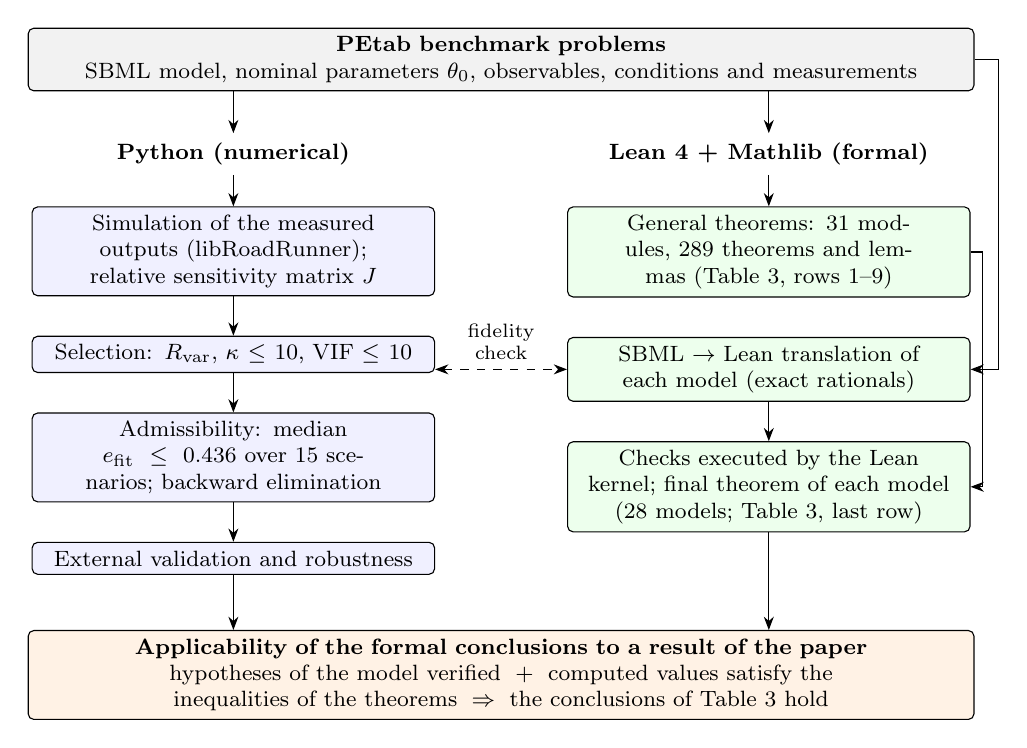
\begin{tikzpicture}[
  font=\footnotesize, >=Stealth, node distance=5mm,
  box/.style={draw, rounded corners=2pt, align=center, inner sep=3pt, text width=#1},
  box/.default=4.9cm]
\node[box=11.8cm, fill=gray!10] (in) at (0,0) {\textbf{PEtab benchmark problems}\\ SBML model, nominal parameters $\theta_0$, observables, conditions and measurements};
\node[font=\footnotesize\bfseries] (py) at (-3.4,-1.2) {Python (numerical)};
\node[font=\footnotesize\bfseries] (lean) at (3.4,-1.2) {Lean 4 + Mathlib (formal)};
\node[box, fill=blue!6, below=4mm of py] (p1) {Simulation of the measured outputs (libRoadRunner); relative sensitivity matrix $J$};
\node[box, fill=blue!6, below=of p1] (p2) {Selection: $R_{\mathrm{var}}$, $\kappa\le10$, VIF $\le10$};
\node[box, fill=blue!6, below=of p2] (p3) {Admissibility: median $e_{\mathrm{fit}}\le0.436$ over 15 scenarios; backward elimination};
\node[box, fill=blue!6, below=of p3] (p4) {External validation and robustness};
\node[box, fill=green!7, below=4mm of lean] (l1) {General theorems: 31 modules, 289 theorems and lemmas (Table 3, rows 1--9)};
\node[box, fill=green!7, below=of l1] (l2) {SBML $\to$ Lean translation of each model (exact rationals)};
\node[box, fill=green!7, below=of l2] (l3) {Checks executed by the Lean kernel; final theorem of each model (28 models; Table 3, last row)};
\node[box=11.8cm, fill=orange!10, anchor=north] (out) at ($(p4.south -| 0,0)+(0,-0.7)$) {\textbf{Applicability of the formal conclusions to a result of the paper}\\ hypotheses of the model verified \;$+$\; computed values satisfy the inequalities of the theorems \;$\Rightarrow$\; the conclusions of Table 3 hold};
\draw[->] (in.south -| py) -- (py.north);
\draw[->] (in.south -| lean) -- (lean.north);
\draw[->] (py) -- (p1); \draw[->] (lean) -- (l1);
\draw[->] (p1) -- (p2); \draw[->] (p2) -- (p3); \draw[->] (p3) -- (p4);
\draw[->] (l2) -- (l3);
\draw[->] (in.east) -- ++(0.3,0) |- (l2.east);
\draw[->] (l1.east) -- ++(0.15,0) |- (l3.east);
\draw[<->, dashed] (p2.east |- l2.west) -- node[above, font=\scriptsize, align=center]{fidelity\\check} (l2.west);
\draw[->] (p4.south) -- (p4.south |- out.north);
\draw[->] (l3.south) -- (l3.south |- out.north);
\end{tikzpicture}
\end{document}
